\documentclass[10pt,journal,compsoc]{IEEEtran}


% ------------------ 加入中文套件 ---------------
\usepackage{xeCJK}
\setCJKmainfont{SimSun}
%----------------------------------------------

%------------------- 图片 ---------------------
\usepackage{graphicx}
\usepackage{caption}
%----------------------------------------------


\usepackage{indentfirst}

\setlength{\parindent}{2em}

\ifCLASSOPTIONcompsoc
\usepackage[nocompress]{cite}
\else
  \usepackage{cite}
\fi

\ifCLASSINFOpdf
\else  
\fi



\hyphenation{op-tical net-works semi-conduc-tor}


\begin{document}
\title{深度学习神经网络}

\author{王成        
\IEEEcompsocitemizethanks{\IEEEcompsocthanksitem  北京市海淀区学院路30号北京科技大学计算机与通信工程学院\protect\\
E-mail: 378716031@qq.com
}
\thanks{成稿于2016年3月21日}}


\markboth{March~2016}%
{Shell \MakeLowercase{\textit{et al.}}}



\IEEEtitleabstractindextext{
\begin{abstract}
《Deep Learning in neural networks》这篇文章是深度学习神经网络方面的一个比较著名的综述型文章,作者主要在其中对深度学习、监督学习、无监督学习。强化学习和进化计算等内容做了不同的概述。然后扼要重述了反向传播和神经网络深度学习的一些历史。
\end{abstract}

\begin{IEEEkeywords}
深度学习、监督学习、无监督学习、神经网络、反向传播、强化学习
\end{IEEEkeywords}}


\maketitle



\IEEEdisplaynontitleabstractindextext

\IEEEpeerreviewmaketitle



\IEEEraisesectionheading{\section{引言}\label{sec:introduction}}

\IEEEPARstart { }《Deep Learning in neural networks》这篇综述,然后对整个文章的脉络做一个回顾,说明通过这篇文章,对深度学习和神经网络的一些理解,以及什么是强化学习,什么是监督/无监督学习等等。

 
\hfill March 21, 2016

\section{概述}这篇文章大概是分成七个部分,首先是对神经网络和深度学习做了一个介绍,让我们了解什么是深度学习,什么是神经网络;然后介绍了通过激活面向事件的符号,使其在神经网络中进行传播;第三部分着重对信用分配路径(CAP)和其面临的一些困难做了介绍;第四部分是对深度学习理论再现,来说明其中一些思想,比如动态规划监督学习,奥卡姆剃刀定律等等;第五部分是对1940至2014年深度学习和神经网络的一些成果以及发展;第六部分的重点放在了强化学习和监督/无监督学习之上;最后底气部分则对整篇文章做了一个总结。

\subsection{深度学习和神经网络}
深度学习的概念源于人工神经网络的研究。含多隐层的多层感知器就是一种深度学习结构。深度学习通过组合低层特征形成更加抽象的高层表示属性类别或特征,以发现数据的分布式特征表示。\par
深度学习的概念由Hinton等人于2006年提出。基于深信度网(DBN)提出非监督贪心逐层训练算法,为解决深层结构相关的优化难题带来希望,随后提出多层自动编码器深层结构。此外Lecun等人提出的卷积神经网络是第一个真正多层结构学习算法,它利用空间相对关系减少参数数目以提高训练性能。\par
同机器学习方法一样,深度机器学习方法也有监督学习与无监督学习之分.不同的学习框架下建立的学习模型很是不同.例如,卷积神经网络(Convolutional neural networks,简称CNNs)就是一种深度的监督学习下的机器学习模型,而深度置信网(Deep Belief Nets,简称DBNs)就是一种无监督学习下的机器学习模型。\par
深度学习的核心思想是:
\begin{itemize}
\item 无监督学习用于每一层网络的pre-train;
\item 每次用无监督学习只训练一层,将其训练结果作为其高一层的输入;
\item 用自顶而下的监督算法去调整所有层。
\end{itemize}\par
人工神经网络:是一种应用类似于大脑神经突触联接的结构进行信息处理的数学模型。神经网络没有一个严格的正式定义。它的基本特点,是试图模仿大脑的神经元之间传递,处理信息的模式.而神经元是神经网络的基本单位。本质上,神经元有着树突、细胞体和轴突。它最重要的特性就是学习。\par
每个神经细胞通过它的树突和大约10,000个其他的神经细胞相连。这就使得你的头脑中所有神经细胞之间连接总计可能有l00,000,000,000,000个。这比100兆个现代电话交换机的连线数目还多。所以毫不奇怪为什么我们有时会产生头疼毛病!\par
曾经有人估算过,如果将一个人的大脑中所有神经细胞的轴突和树突依次连接起来,并拉成一根直线,可从地球连到月亮,再从月亮返回地球。如果把地球上所有人的脑中的神经细胞的轴突和树突连接起来,则可以伸展到离开我们最近的星系!\par
由于数量巨大的这些连接,使得我们大脑可以完成许多难以置信的功能。
\begin{itemize}
\item 能实现无监督学习(这点在神经网络中尤为重要)
\item 对损伤有冗余(tolerance)
\item 处理信息的效率是非常高的
\item 善于对事物进行归纳和推广 
\item 有意识
\end{itemize}

神经网络要做的,其实就是要尽可能的在目前硬件的条件下来模拟这种并行性,并在实现过程中表现出与人类大脑相似的特性。

\subsection{深度学习理论的再现}
\subsubsection{对监督/强化学习进行动态规划}
动态规划需要系统模型,它的优点主要是几乎不需要对系统做任何的假设,可以具有非线性和随机性。动态规划构造模拟模型比衍生一个解析模型要容易许多,特别是对随机的情况来说。而强化学习由于代价太大,事先无法对系统做全面的感知,所以其并不需要系统模型。强化学习的优点是他是从系统中得到的数据来工作,并不需要行为模型。\par
强化学习和动态规划问题的主要要素是通过他们之间的交流相互联系在一起:首先是过程为控制器提供目前所处的状态;其次控制器根据目前的状态,为过程提供应采取的动作;最后过程再给出下一状态,并根据奖赏函数,给出其获得的立即奖赏。\par
在强化学习和动态规划中,目标是使回报最大化,其中回报是由交互过程中的累积奖赏所构成。
\subsubsection{无监督学习和有监督学习}
首先看这两个概念,是否有监督,就看输入的数据是否有标签。有标签的是有监督学习,否则是为无监督学习。\par
在机器学习算法中,分类是最简单最普遍的一类算法之一。对于分类,输入的训练数据有特征、有标签。而学习的本质是找到特征与标签之间的关系。这样当有特征而无标签的未知数据输入时,我们就可以通过已有的关系得到未知的数据标签。\par
在上述的分类过程中,如果所有训练数据都有标签,则为有监督学习(supervised learning)。如果数据没有标签,显然就是无监督学习(unsupervised learning)了,也即聚类(clustering)。\par
通俗的说来,监督学习是指我们来教计算机如何“学习”,非监督学习是指让计算机自己学习。\par
无监督学习还有一个典型的例子就是鸡尾酒会问题(声音的分离),在这个酒会上有两种声音,被两个不同的麦克风在不同的地方接收到,而可以利用无监督学习来分离这两种不同的声音。注意到这里是无监督学习的原因是,事先并不知道这些声音中有哪些种类(标签)。
\subsubsection{奥卡姆剃刀定律}
这个原理是14世纪由圣方济各会修士奥卡姆 威廉提出,原理的内容称为:Entities should not be multiplied unnecessarily。一般常用于两种或两种以上假说的取舍上:如果对于统一现象有两种或多种不同的假说,我们应采取比较简单或可证伪的那一种,世界客观存在即是建立在客观实践之上,正所谓实践是检验真理的唯一标准。\par
在神经网络领域中对奥卡姆地道定律的应用主要是在归纳偏置上。当学习器去预测其从未遇到过的输入的结果时,会做一些假设,而学习算法中归纳偏置则是这些假设的集合。\par
那么,什么是归纳偏置?机器学习试图去建造一个可以学习的算法,用来预测某个目标的结果。要达到此目的,要给于学习算法一些训练样本,样本说明输入与输出之间的预期关系。然后假设学习器在预测中逼近正确的结果,其中包括在训练中未出现的样本。既然未知状况可以是任意的结果,若没有其它额外的假设,这任务就无法解决。这种关于目标函数的必要假设就称为归纳偏置。\par
一个典型的归纳偏置例子就是奥卡姆剃刀,他假设最简单而又一致的假设是最佳的。这里的一致是指学习器的假设会对所有样本产生正确的结果。

\subsection{有监督神经网络有助于无监督神经网络}
这一部分主要是从1940年至2014年的一些事件或例子上可以看出:
\begin{itemize}
\item 1940年,早期神经网络开始出现
\item 1960年,视觉皮层为深度学习提供了灵感
\item 1965年,基于数据分组处理方法的深度网络
\item 1979年,卷积+权重复制+二次抽样(神经认知机)
\item 1960-1981,反向传播算法的发展
\item 1989年,卷积神经网络的反向传播
\item 1991:梯度下降的根本性深度学习问题
\item 1994年,神经网络获得早期一些比赛的胜利
\item 2003年,神经网络成为更多大赛的冠军,缔造了多项记录
\item 2009年,递归神经网络联合最大池卷积神经网络赢得比赛胜利
\end{itemize}
等等各项内容,一一说明了神经科学的重要性。



\subsection{深度学习在前馈神经网络和递归神经网络中的强化学习}
深度学习方法促进了人工神经网络的发展,它在传统的人工神经网络训练中增加了一个预训练阶段,即用无监督学习对每一层网络进行一次专门的训练,然后才用有监督学习对整个网络进行总体训练。\par
通过深度学习方法,人工神经网络的效果一举赶上甚至显著超过了支持向量机等其他机器学习方法。
\subsubsection{通过对神经网络模式的强化学习,产生了深度信用分配路径的递归神经网络}
首先介绍还前馈神经网络(FNN),简称前馈网络,是人工神经网络的一种。在此种神经网络中,各神经元从输入层开始,接收前一级输入,并输入到下一级,直至输出层。整个网络中无反馈,可用一个有向无环图表示。它是最早被提出的人工神经网络,也是最简单的人工神经网络类型。按照前馈神经网络的层数不同,可以将其划分为单层前馈神经网络和多层前馈神经网络。常见的前馈神经网络有感知机(Perceptrons)、BP(Back Propagation)网络、RBF(Radial Basis Function)网络等。前馈神经网络图如Fig.1:\par

\makeatletter
\def\@captype{figure}
\makeatother

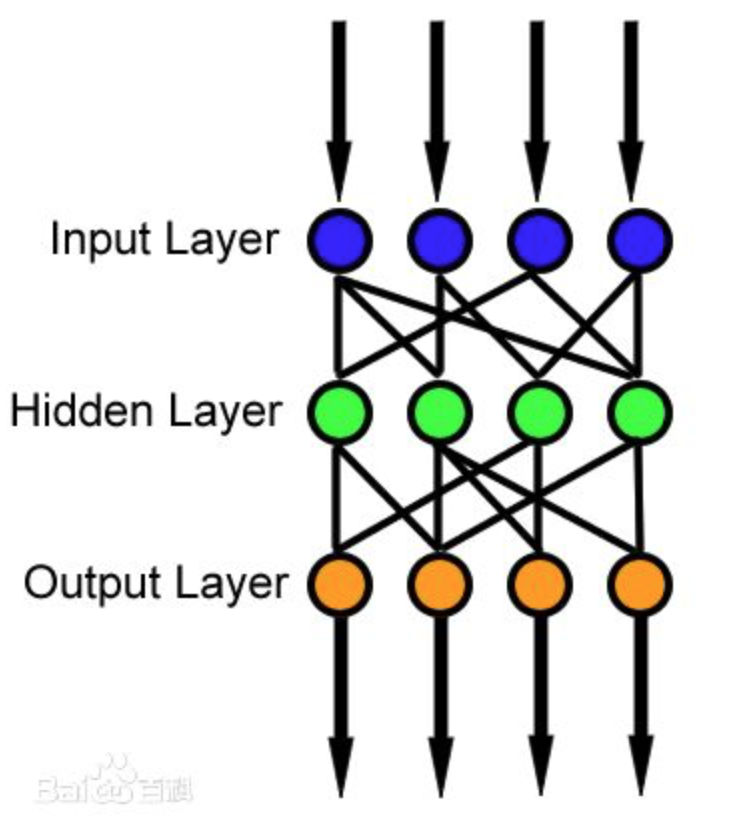
\includegraphics[width = .4\textwidth]{feedback.png}
\caption{前馈神经网络}
在强化学习前馈神经网络控制器C与一个确定性的,有预见性的运行环境进行交互的特殊事例中,一个单独的称为M的前馈神经网络可以学习去变成C的模式,来通过系统的确认,其可以预见的输入来自与其先前的行为和输入。假设M已经学会去产生精确的预测。我们可以使用M来替代运行环境。于是M和C形成一个递归神经网络,而M的输出变成了C的输入,其输出(行为)反过来成了M的输入。现在,对递归神经网络的反向传播可以用于实现渴望输入的事件,诸如高实值奖励信号:一旦M的权重保持不变,C权重的梯度信息会通过M传回至C,再传回M等等。在一定程度上,这个方法也适用于概率和不确定的环境下,只要M的基于C的梯度估计的内积和M的“真实”梯度趋向于一个确定值。

\subsubsection{深度前馈神经网络的传统强化学习和马尔可夫决策过程}
马尔可夫决策过程(MDPs)以安德烈马尔可夫的名字命名 ,针对一些决策的输出结果部分随机而又部分可控的情况,给决策者提供一个决策制定的数学建模框架。MDPs对通过动态规划和强化学习来求解的广泛的优化问题是非常有用的。更确切地说,一个马尔可夫决策过程是一个离散时间随机控制的过程。在每一个时阶(each time step),此决策过程处于某种状态 s ,决策者可以选择在状态 s 下可用的任何动作 a。该过程在下一个时阶做出反应随机移动到一个新的状态 s',并给予决策者相应的奖励 Ra(s,s')。此过程选择 s'作为其新状态的概率又受到所选择动作的影响。马尔可夫决策过程是一个马尔可夫链的扩展;区别是动作(允许选择)和奖励(给予激励)的加入。相反,如果忽视奖励,即使每一状态只有一个动作存在,那么马尔可夫决策过程即简化为一个马尔可夫链。\par
经典的强化学习的方法,使马尔可夫决策过程的假设简单化:强化学习代理的输入电流输送所需的全部信息到最佳的下一个输出事件或决策。这允许使用动态编程技巧来大大减少信用分配路径在强化学习神经网络中的深度。后者通常是在概率框架中解释的,但它基本的思想已经可以用一个确定的设置来传达。\par

\subsubsection{通过在FNNs和RNNs中加深无监督学习来使强化学习更便利}
强化学习机可以从输入过程的无监督学习中受益。特别的,一个无监督学习神经网络可以学着紧凑地编码环境输入如同图像和视频,等等。\par
紧凑的代码(而不是高维未处理数据)可以被送入一个强化学习机,其工作可能因此变得更加容易,就像监督学习可能从无监督学习中受益。例如,神经嵌合的Q学习算法已经应用于真实世界的控制任务。其中,纯粹的视觉输入是通过深度自编码器进行的紧凑编码。基于慢特征分析的强化学习与无监督学习的结合,使一个真正的人形机器人从原生高维视频流中学本事。为了应对部分可观察的马尔可夫决策过程涉及的高维输入,基于受限玻尔兹曼机的强化学习和递归自联想记忆作为一个深度的无监管序列编码器为强化学习所使用。某些强化学习和无监督学习的类型也合并在生物学上似乎有理的递归神经网络尖峰神经元上。
\subsubsection{前馈神经网络和递归神经网络的深度分层学习和子目标学习}
多重可学习抽象概念的水平似乎认为强化学习和监督学习同样很重要,基于神经网络的分层强化学习的工作自90年代初已经发布。特别是,基于梯度的前馈神经网络或递归神经网络的子目标发现分解强化学习任务为子任务的强化学习子模块。众多替代分层强化学习的技术已经被提出。虽然分层强化学习框架,如传统强化学习和选项不直接处理自动发现子目标的问题,HQ-学习将在简单子任务序列中自动分解部分可观察的马尔可夫决策过程,这可以通过反应副剂记忆策略学习来解决。最近分层强化学习组织潜在的深度基于神经网络的强化学习子模块集成到自我的组织,由神经生理学的研究结果产生了二维马达控制图。
\subsubsection{通过直接神经网络搜索/策略梯度/进化进行深度强化学习}
既实用又比大多数传统强化学习算法更普遍的,是直接策略搜索的方法,而不需要值函数或马尔可夫假设,前馈神经网络或递归神经网络的权重直接评估在给定的强化学习的问题上。连续实验的结果通知进一步的寻找更好的权重。不同于反向传播所支持的强化学习,信用分配路径的深度并不是一个关键的问题。直接策略搜索可以解决信用分配的问题而不用经过修改深因果链条参数来回溯——它既不关心自己的存在,也不试图应用他们。\par
对神经网络直接策略搜索的方法是一类重要的策略梯度法。经过反复的神经网络评估,考虑了政策的总报酬的梯度已经被估计了出来。\par
强化学习神经网络也可以通过进化算法的一系列试验逐步发展而来。这儿的若干政策是通过神经网络群经过突变和/或人口的适者生存的不断重组来改善的。比较那些可用于进化可变型号的计算机程序的遗传编程,和笛卡尔遗传编程在图形化编程上的不断发展,包括神经网络和他们的拓扑结构。相关的方法包括基于概率分布的进化算法,协方差矩阵估计进化策略,和增光拓扑的神经元进化。混合的方法结合了传统的基于神经网络的强化学习和进化算法。\par
因为递归神经网络是一般的计算机,递归神经网络的发展感觉像是基因编码,他可以进行一般化的编程。不同于由传统基因编码学习到的顺序编程,然而,递归神经网络可以以一个自然并且有效的方式混合顺序和并行的信息处理,就像在Section1中提到的那样。许多递归神经网络的先驱者已经提了出来,一个特殊的、有效的方法簇共同进化神经元,它们组合成网络,并选择了那些参与进最佳网络的神经元用于再生。这可以帮助解决深度部分可观察马尔可夫决策。联合突触神经进化确实在突触或权重的水平上有一些类似;这个好处是显示了困难的非线性部分可观察马尔可夫决策的基准。\par
\subsubsection{通过间接神经策略搜索/压缩的神经网络搜索进行深度强化学习}
有些直接政策搜索方法可以演变成成千上万权重,而不是数百万权重的神经网络。如何寻找又大又深的神经网络?大多数监督学习和强化学习的方法到目前为止以某种权重的搜索空间的方式被提及过了。一些通过减少共享无线搜索空间而获得的利润,在卷积神经网络或在递归神经网络的监督和强化学习中被一遍又一遍重复使用。
这是可能的,无论如何,利用附加的规律性/压缩性溶液中的空间,通过在权重空间中的间接搜索。而不是直接进化成大型神经网络。有时课通过Lindenmeyer系统,图表重写,蜂窝编码,超级NEAT和对他们的扩展,通过发展间接的神经网络编码来极大的减少搜索空间。这有助于避免正规化的主题和马尔可夫决策的过度拟合和密切相关。
为监督学习和强化学习的一般化方法试图通过编写一个通用的编程语言来使大型神经网络的编码权重变得紧凑。有条理的对一些倾向性的短期和快速程序的空间进行搜索往往更有效率,而不是直接寻找可能的神经网络权重矩阵的巨大空间。编码神经网络先前的通用语言是类汇编语言。最近的工作使用更实用的基于流行变换系数的语言。特别是,递归神经网络权重矩阵通过余弦函数变换编码他们,可使其被压缩成类似图像。压缩的基于离散余弦变换的描述可以通过NES(自然进化策略)或者CoSyNE(联合突触神经进化)发展。超过100万权重的递归神经网络以高维视频一般的视觉输入流为基础,学会了(没有老师)在TORCS驾驶游戏上驾驶模拟汽车。该递归神经网络从头学会了控制和视觉处理,无需无监督学习的帮助。(当然,无监督学习可能帮住产生更紧凑的图像代码)来馈送进一个较小的递归神经网络,来减少整个的计算量)。


\subsubsection{通用强化学习}
一般目的学习算法可以在一个终身学习背景下以开放的方式和具体的环境来提高他们自己。强化学习的最普遍类型是受限的,这种限制仅由理论计算机科学的奠基人确定其可计算性的根本局限性而确认。值得注意的是,他们存在通用问题解决者或通用强化学习机的蓝图,用于绝对的问题深度,这种深度是在各种理论意义下的时间优化。特别的,哥德尔机器可以在通用计算机,例如递归神经网络上实现,并且可能以一定意义上对时间优化的方式提高其软件的任何部分(包括算法学习本身)。他可以通过一个渐进最优元方法初始化(同样适用于递归神经网络),这将解决任何明确定义的问题就像解决未知的最快方式一样快,保存为一个额外的常数开销,这个开销作为问题规模的增长可忽略不计。注意,大多数问题比较严重,只有少数的很小。人工智能和深度学习的研究人员仍旧在企业,因为有许多小的有意思的问题,值的去尝试通过减少一般方法来降低开销,包括启发式。这里,并不会深入讨论普遍的强化学习方法,这超出了我们通常所说的深度学习范围。





\section{结论}
深度学习在神经网络中与监督学习、非监督学习和强化学习相关。通过减轻深度信用分配路径的问题,无监督学习不仅有利于连续的监督学习和固定的模式,还有利于强化学习。动态编程对深度监督学习和传统神经网络强化学习很重要。一种用于解决计算性、抗扰动,低复杂度神经网络的搜索通过较少信息位的描述,可以减少过度拟合和改善深度监督,无监督学习还有强化学习,也在这个部分可观察环境的事例下。深度的监督学习、无监督学习、强化学习通常创建平稳数据,连续数据或强化学习政策的越来越抽象表示层次结构。前馈神经网络中的深度学习在GPU(图形处理单元)实现中获益良多。特别是,基于图形处理单元的最大池卷积神经网络不仅在模式识别中赢得比赛,还在图像分割和对象见侧重获胜。\par
与这些系统不同,人类学会通过有序的将注意力集中到现有数据的相关部分来主动的感知图像。不久的将来深度神经网络也会做到这一点,在通过电动机动作的强化学习来学习选择性注意的神经网络,如扫视控制和通过递归神经网络内部行为控制注意力的光线。从而通过两个内外的反馈来贴近这个通用的聚光环。
未来的许多深层神经网络也将考虑他激活神经元,并在他们之间传送信号的能量成本。\par
论文作者认为更远的将来可能属于通用学习算法,这种算法可以以一种可证明的最佳方式改善自身,这些还并不实用或并没有进行商用。但目前最新的进展来看,已经进行了商业推广。


\appendices
\section{文中出现的一些神经网络缩略词}
\begin{itemize}
\item 信度分配路径(Credit Assignment Path,CAP)
\item 深度学习(Deep Learning,DP)
\item 动态规划(Dynamic Programming,DP)
\item 前馈神经网络(Feedforward Neural Network,FNN)
\item 图像处理单元(Graphics Processing Unit,GPU)
\item 最大池卷积神经网络(Max-Pooling Convolutional Neural Network,MPCNN)
\item 长短期记忆(Long-Short Term Memory,LSTM)
\item 最小描述长度(Minimum Description Length,MDL)
\item 马尔科夫决策过程(Markov Decision Process,MDP)
\item 神经网络(Neural Network,NN)
\item 部分可观测的马尔科夫决策过程(Partially Observable MDP,POMDP)
\item 受限玻尔兹曼机(Restricted Boltzmann Machine,RBM)
\item 强化学习(Reinforcement Learning,RL)
\item 递归神经网络(Recurrent Neural Network,RNN)
\item 弹性反向传播(Resilient Backpropagation,R-prop)
\item 监督学习(Supervised Learning,SL)
\item 无监督学习(Unsupervised Learning,UL)
\end{itemize}



\newpage
\ifCLASSOPTIONcompsoc
  \section*{致谢}
\else
  \section*{致谢}
\fi
首先感谢罗熊老师的谆谆教导,让我们在四周的有限时间里对LaTex做了一些了解,并在罗老师的指导下进行了深度学习论文的翻译、研讨。\par
还要感谢和我同一小组的几位同学,是你们和我一起探讨问题,并指出我观点上的误区,使我能及时的发现问题把论文顺利的进行下去,没有你们的帮助我不可能这样顺利地结稿,在此表示深深的谢意。\par
最后感谢众多热心网友的Latex技巧的无私奉献和在深度学习方面对我有启蒙意义的论文作者Jürgen Schmidhuber。


\ifCLASSOPTIONcaptionsoff
  \newpage
\fi

\begin{thebibliography}{1}

\bibitem{IEEEhowto:kopka}
Jürgen Schmidhuber, \emph{Deep learning in neural networks: An overview}, 61:85 - 117,2015.

\end{thebibliography}


\begin{IEEEbiography}[{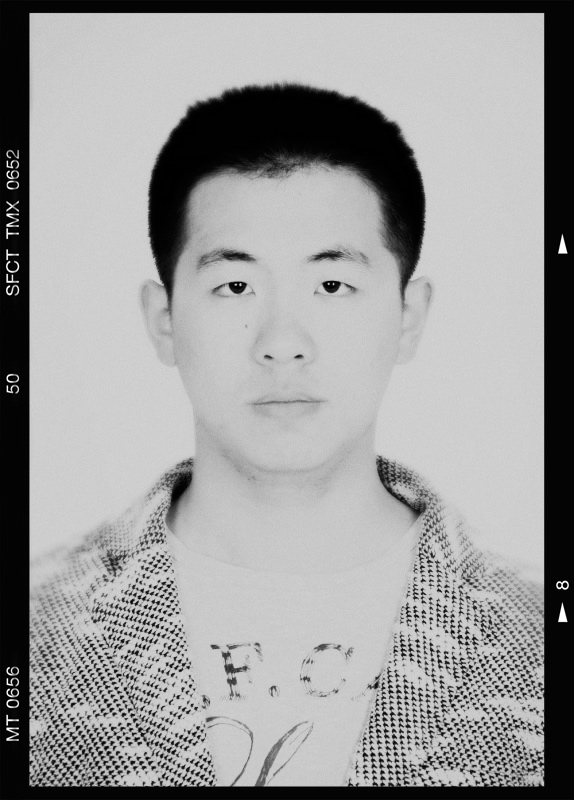
\includegraphics[width=1in,height=1.25in,clip,keepaspectratio]{wang.jpg}}]{王成}
(1990 - )北京科技大学计算机与通信工程学院中瑞合作研究生,软件工程与交互设计专业。
\end{IEEEbiography}


\end{document}


